\documentclass[12pt]{article}

\usepackage{sbc/sbc-template}
\usepackage{graphicx,url}
\usepackage[brazil]{babel}
\usepackage[utf8]{inputenc}


\sloppy

% Metadata
\title{Análise Técnica de Arquiteturas de Software no desenvolvimento de aplicativos para Smartphones}
\author{João Pedro Pereira Lemos\inst{1}, Igor Rafael Silva Valente\inst{1}}
\address{Instituto Federal de Educação, Ciência e Tecnologia do Estado do Ceará (IFCE)
  \email{joao.pedro.pereira62@aluno.ifce.edu.br, igor@ifce.edu.br}
}

\begin{document} 

\maketitle

% Abstract
\begin{abstract}
  When creating applications for smartphones, developers make important decisions that directly impact the long-term growth of a project.
The software architecture is a determining factor for the success of an application.
It is of paramount importance that this is well defined, and has characteristics that allow its evolution and maintenance in a sustainable way.
This work compares two common development approaches, discussing their characteristics.
The MVC pattern is compared with the Clean Architecture, using the scenario-based analysis of software architecture.
The main contribution of this paper is to provide an analysis of the architectures chosen in an application for smartphones.
\end{abstract}
     
\begin{resumo}
  Ao criar aplicações para smartphones, os desenvolvedores tomam decisões importantes que impactam diretamente no crescimento de um projeto no longo prazo.
A arquitetura de software é um fator determinante para o êxito de um aplicativo.
É de suma importância que esta seja bem definida e possua características que permitam sua evolução e manutenção de maneira sustentável.
Este trabalho compara duas abordagens de desenvolvimento amplamente empregadas, analisando suas características.
O padrão MVC é comparado com a Arquitetura Limpa, utilizando o método de análise de arquiteturas de software baseado em cenários.
A principal contribuição deste artigo é fornecer uma análise das arquiteturas escolhidas em uma aplicação para smartphones.
\end{resumo}


% Introduction
\section{Introdução}

Os smartphones fazem parte do cotidiano da sociedade, de modo que muitas tarefas podem ser realizadas por intermédio deles.
Comunicação, entretenimento, notícias, educação, saúde, serviços, entre outros.
As operações por meio de smartphones já representam mais de 51\% das transações bancárias no Brasil.
Empresas do setor financeiro estão investindo muito neste segmento.
Estima-se que só em 2020 foram aplicados mais de R\$ 25,7 bilhões~\cite{febraban-data}.
Segundo uma pesquisa realizada em 2022, existem 447 milhões de dispositivos digitais em uso no Brasil, sendo 242 milhões destes, smartphones.
Há mais de 1 smartphone por habitante em território nacional~\cite{it-usage-data}.
O Banco Central do Brasil estabeleceu em 2020 um novo meio de pagamento — o Pix.
Esse meio de pagamento nasceu com a ideia de utilizar o smartphone para enviar e receber dinheiro, dada a sua massiva utilização.
Apenas no mês março de 2022, mais de 784 milhões de transações foram realizadas por meio do Pix~\cite{pix-statistics}.

Dada a importância que os smartphones têm na sociedade, é importante garantir que as aplicações desenvolvidas tenham um padrão de qualidade.
Empresas de tecnologia estão preocupadas com o \emph{time to market}, termo que designa o tempo decorrido desde a concepção da ideia até a publicação de um produto.
Assim, diversas abordagens são utilizadas para entregar o produto no menor tempo possível, em muitos casos sacrificando a qualidade, e causando débitos técnicos dentro do projeto.
Em geral, nota-se que mudanças na regra de negócio e eventuais adições de funcionalidades podem ter uma complexidade maior quando a arquitetura do projeto é muito permissiva, ou não é bem definida.
A garantia de qualidade muitas vezes está concentrada apenas no processo de QA, e o código-fonte produzido não é levado em consideração.
Nem tudo pode ser prevenido, e \emph{bugs} geralmente são um reflexo disso~\cite{quality-standards-paper}.

O presente artigo compara duas abordagens diferentes para se desenvolver um aplicativo para smartphones, analisando como se comportam em face à evolução do software.
Inicialmente, são apresentados trabalhos de outros autores que se relacionam com o tema escolhido.
Depois, os conceitos de Engenharia de Software que permearão este trabalho são discorridos brevemente.
Na sequência a metodologia adotada é apresentada.
Em seguida, o padrão MVC é comparado à Arquitetura Limpa, utilizando método de análise de arquiteturas de software baseado em cenários.
Ao final, são apresentadas as conclusões da análise realizada.


% Related work
\section{Trabalhos relacionados}

\shortciteA{humeniuk} compara a arquitetura VIPER com o MVP, na plataforma Android, com o objetivo de verificar a viabilidade de cada abordagem.
Uma aplicação de notas é desenvolvida em ambas as arquiteturas.
Modificabilidade, testabilidade, manutenabilidade e performance são usadas como métricas para a análise.
O trabalho conclui que ambas as abordagens são viáveis, e que o MVP é mais adequado para projetos pequenos, ao passo que o VIPER é adequado para projetos maiores.

No segundo trabalho, é apresentada uma análise de diversos padrões arquiteturais para o desenvolvimento na plataforma Android.
Abordagens como o MVC, MVP, MVVM, VIPER e a Arquitetura Limpa são comparadas subjetivamente em relação ao acoplamento, coesão, testabilidade e manutenibilidade, investigando qual padrão arquitetural é o mais adequado.
De acordo com o estudo, uma combinação de MVVM com Arquitetura Limpa atingem os atributos desejados.
A comparação não conta com um exemplo real de código para cada abordagem~\cite{akhtar}.

O presente artigo justifica-se por trazer uma análise baseada em cenários, a partir de um projeto de exemplo, em cada uma das abordagens selecionadas.
São considerados aspectos importantes, como a facilidade de implementar novos recursos, o impacto de modificações futuras, possibilidade de modularizar a aplicação, curva de aprendizado de cada abordagem e a facilidade de escrever testes unitários.
Também, a análise realizada é válida tanto no desenvolvimento em plataformas específicas, como o Android e iOS, quanto em frameworks híbridos, como Flutter ou React Native.


% Foundation
\section{Fundamentação teórica}

Padrões arquiteturais são descrições de alto nível dos componentes de um software e seus relacionamentos.
O padrão MVC (\emph{Model-View-Controller}) é apresentado como uma abordagem que visa padronizar a forma que os sistemas com interface gráficas são construídos, dividindo as responsabilidades da aplicação em alguns componentes~\cite{mvc-paper}.

A \emph{Clean Architecture} (Arquitetura Limpa, em português) é uma abordagem que unifica as ideias presentes no \emph{Domain-Driven Design}~\cite{ddd-book} e na \emph{Hexagonal Architecture}~\cite{hexagonal-arch} com os princípios SOLID\@.
A arquitetura visa permitir que o software desenvolvido seja plenamente testável, por desacoplar dependências externas.
Além disso, a arquitetura almeja possibilitar que o cliente da aplicação seja desacoplado da lógica de negócio~\cite{clean-arch-book}.

SOLID é um acrônimo em inglês para 5 princípios de design de software, sendo estes o Princípio da Responsabilidade Única, Princípio do Aberto-Fechado, Princípio da Substituição de Liskov, Princípio da Segregação de Interfaces e Princípio de Inversão de Dependências.
Seu objetivo é guiar a criação de componentes coesos, com um baixo acoplamento, que tolerem mudanças, sejam de fácil entendimento e sirvam de base para a criação outros projetos de software~\cite{clean-arch-book}.

Coesão diz respeito ao relacionamento que os membros de um determinado componente possuem entre si.
Componentes coesos possuem uma relação forte, onde os membros estão intimamente ligados em prol de um objetivo comum.
Acoplamento se refere a quanto um componente é dependente de outro para funcionar corretamente.
Componentes desacoplados tornam a aplicação mais flexível a mudanças, além de torná-los reutilizáveis.
Em geral, componentes com um baixo acoplamento possuem alta coesão, e vice-versa~\cite{coupling-and-cohesion}.


% Methodology
\section{Metodologia}

Para atingir o objetivo deste artigo, foram desenvolvidas duas versões de um mesmo aplicativo de notas, uma utilizando o padrão MVC, e outra utilizando a Arquitetura Limpa.
A aplicação permite o cadastro e autenticação por meio de credenciais ou de uma conta Google.
Após autenticar-se, o usuário é capaz de criar, visualizar, editar e apagar notas que existam em sua conta.
Os dados são armazenados no serviço remoto Firebase \cite{firebase}, além de serem persistidos localmente no dispositivo.
O aplicativo foi construído utilizando a linguagem Dart, fazendo uso do framework Flutter~\cite{flutter}.
Na Figura~\ref{fig:screenshots} é possível visualizar cinco capturas de tela do aplicativo.
A Figura~\ref{fig:project_clean_arch} contém o diagrama da aplicação desenvolvida com a arquitetura limpa, e a Figura~\ref{fig:project_mvc} contém o diagrama da aplicação desenvolvida com MVC.

\begin{figure}[ht]
	\centering
	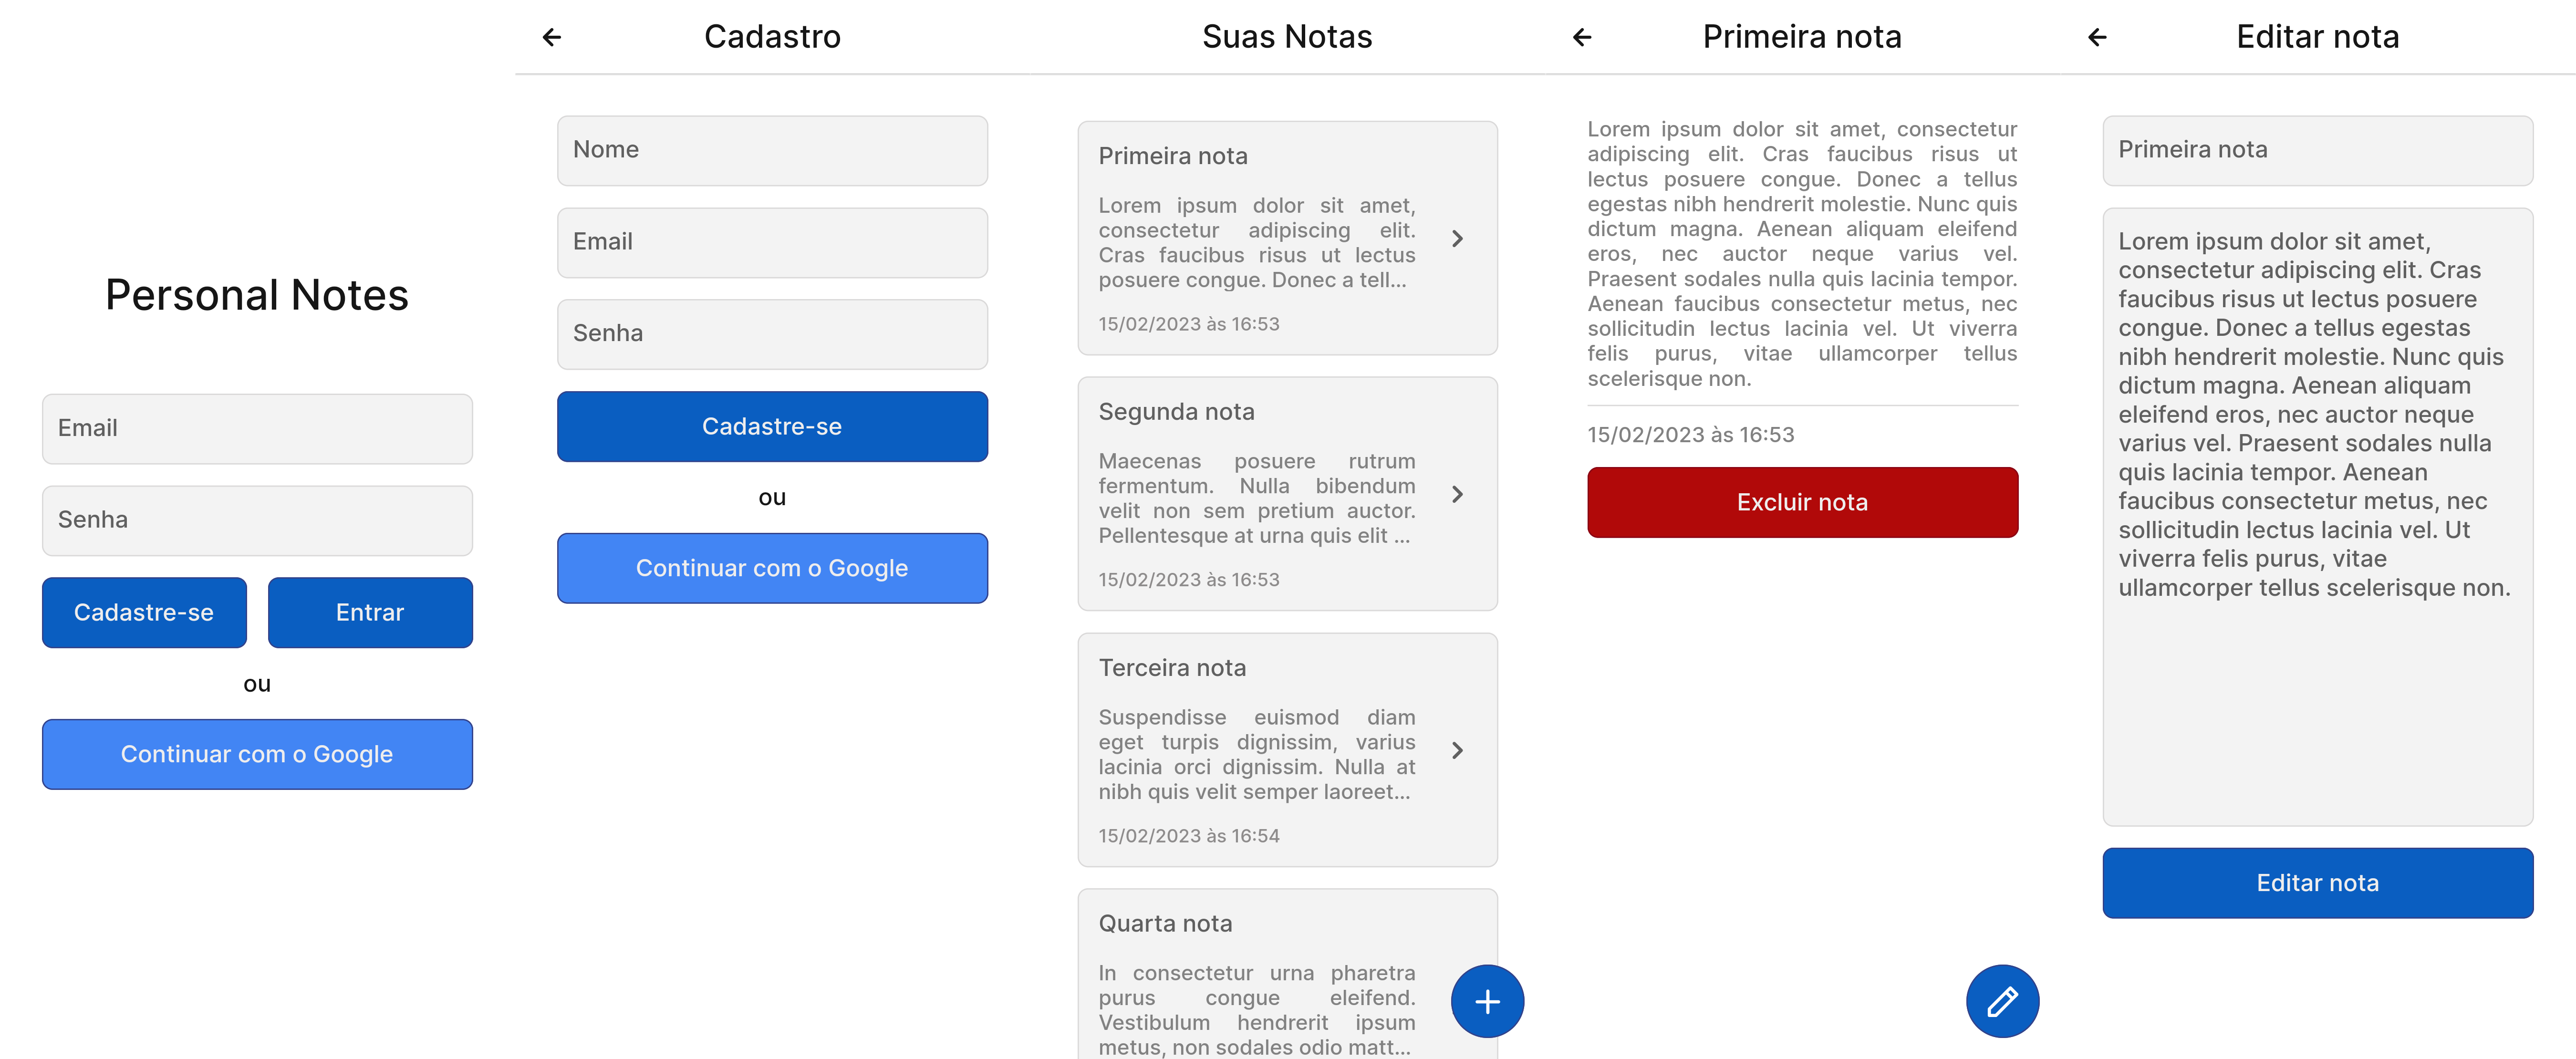
\includegraphics[width=0.8\textwidth]{images/screenshots.png}
	\caption{Capturas de tela do aplicativo}
	\label{fig:screenshots}
\end{figure}

\begin{figure}[ht]
	\centering
	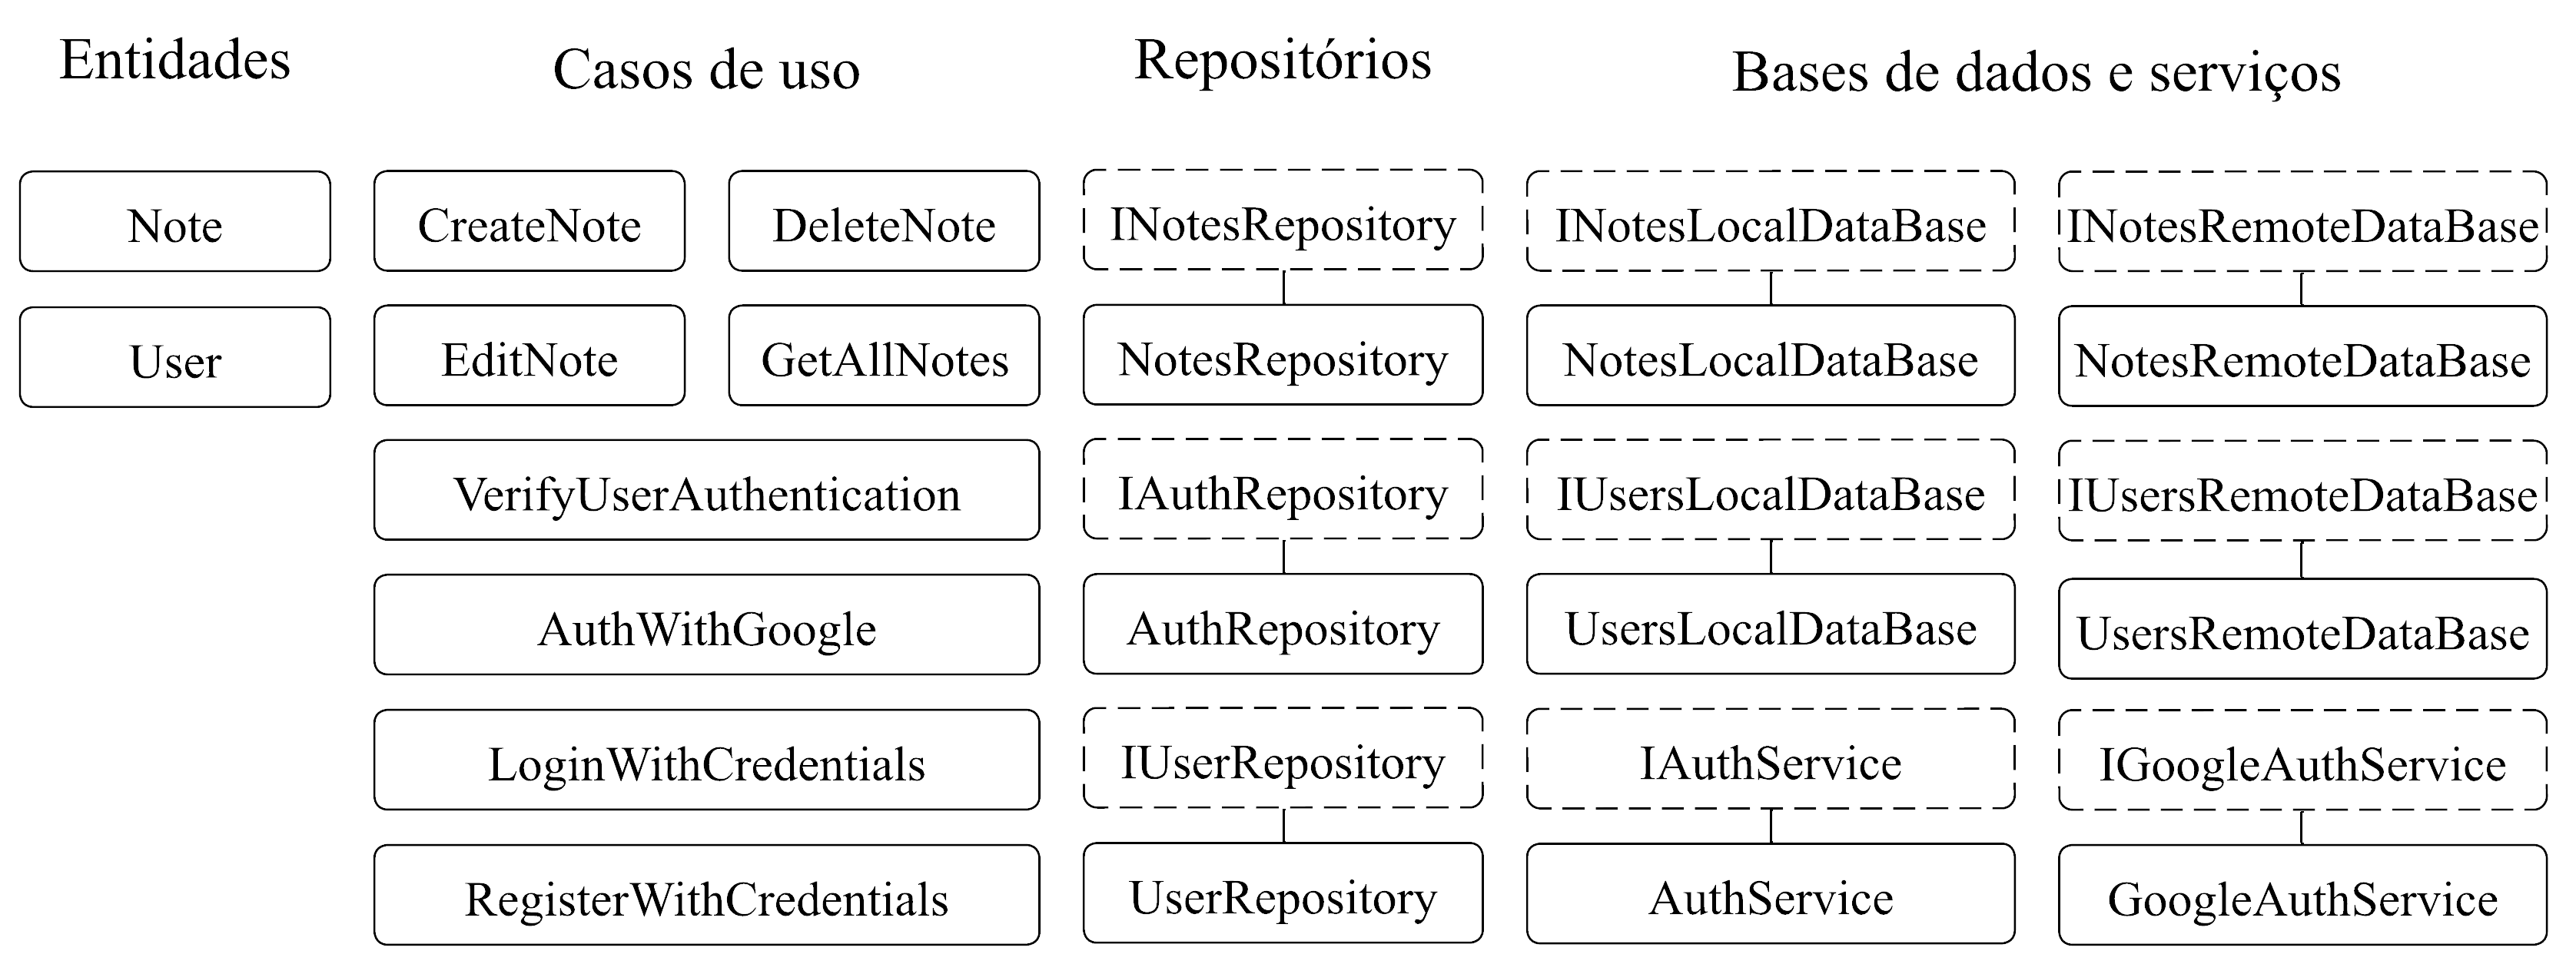
\includegraphics[width=1\textwidth]{images/project_clean_arch.png}
	\caption{Componentes e abstrações do projeto criado com a arquitetura limpa}
	\label{fig:project_clean_arch}
\end{figure}

\begin{figure}[ht]
	\centering
	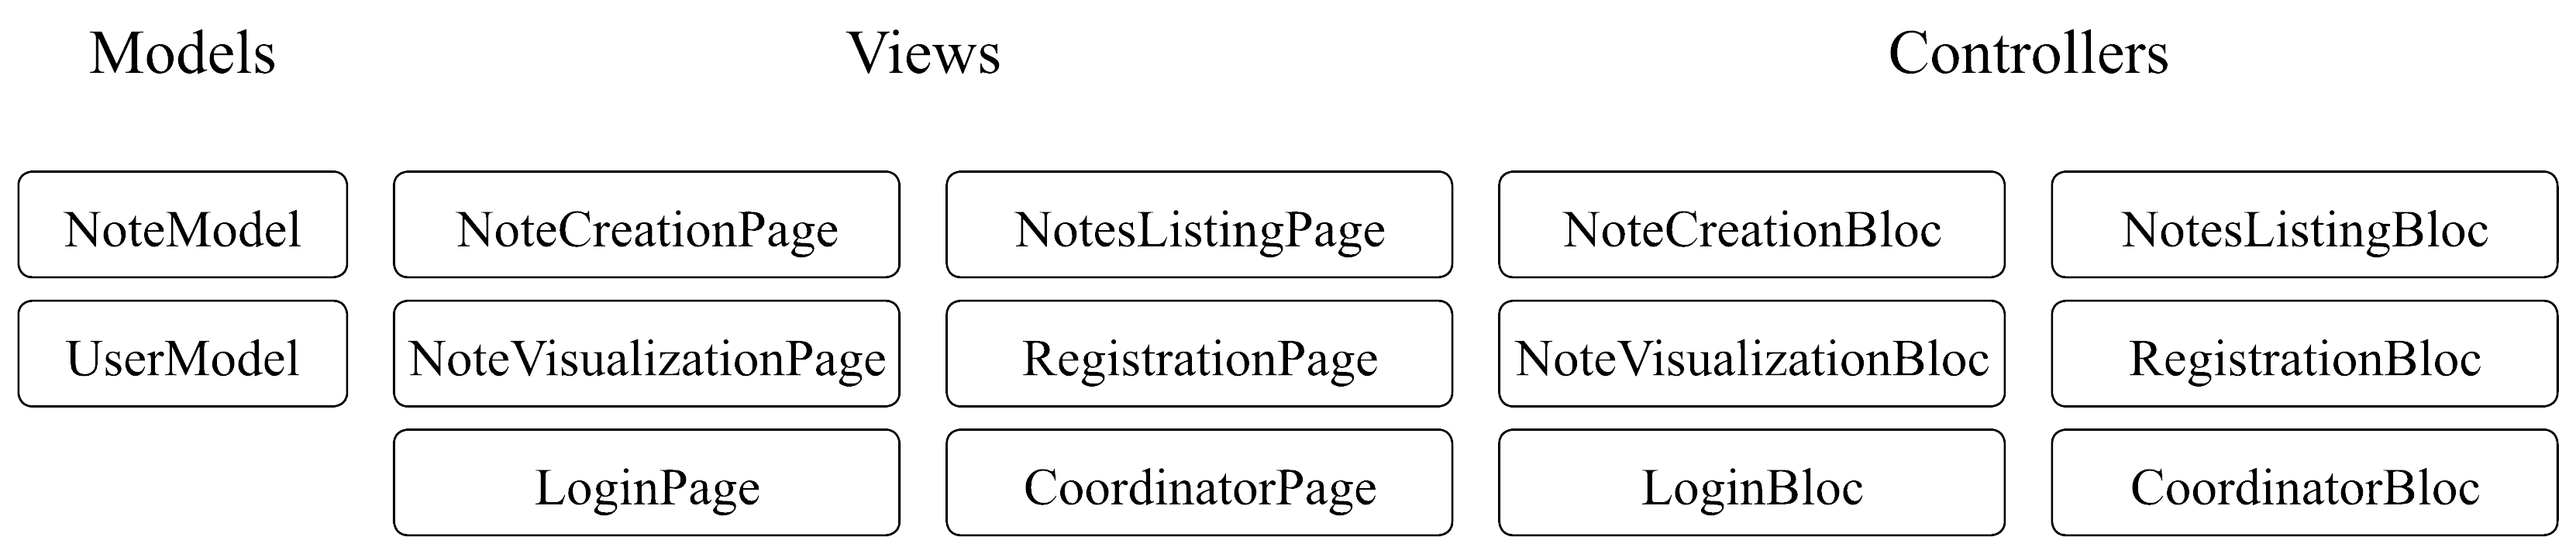
\includegraphics[width=1\textwidth]{images/project_mvc.png}
	\caption{Componentes do projeto criado com MVC}
	\label{fig:project_mvc}
\end{figure}

\subsection{Método de análise de Arquiteturas de Software baseado em cenários}

A análise se dará por meio do método baseado em cenários.
Um cenário é uma breve narrativa de usos esperados ou antecipados do sistema, tanto do ponto de vista do usuário quanto do desenvolvedor.
Ele fornece uma visão de como o sistema satisfaz atributos de qualidade em vários contextos de uso~\cite{scenario-based}.

Inicialmente, é realizada uma descrição da arquitetura candidata.
Após esta etapa, os cenários são desenvolvidos, de modo a ilustrar os tipos de atividades que o sistema deve suportar e as mudanças que são esperadas ao longo da vida de um software.
Então, para cada cenário, é avaliado se a arquitetura necessita de alterações para executar o cenário.
Em caso afirmativo, o cenário é classificado como direto. Caso contrário, é classificado como indireto.

Quando dois ou mais cenários indiretos necessitam de mudanças em algum componente, diz-se que eles interagem.
As interações mostram quais módulos estão envolvidos em quais tarefas.
Um alto nível de interação pode significar que um componente possui um alto acoplamento.

\subsubsection{Cenários propostos}

Serão analisados os seguintes cenários:

\begin{enumerate}
	\item Mudança no banco de dados remoto

	      É desejado que o banco de dados remoto seja substituído, de modo a utilizar a infraestrutura de outro serviço externo.

	\item Implementação da pesquisa de notas por título e conteúdo

	      É desejado que seja possível realizar a pesquisa por notas, tanto no banco de dados remoto quanto no local. Os resultados devem ser apresentados em ordem cronológica.

	\item Implementação de um novo método de autenticação

	      É desejado que seja possível autenticar-se utilizando uma conta do GitHub, além dos métodos já existentes.
\end{enumerate}

\subsection{O padrão MVC (\emph{Model-View-Controller})}

\citeA{mvc-paper} apresenta uma proposta para lidar com conjuntos de dados grandes e complexos dentro de uma aplicação, enquanto permite que a interface de usuário seja atualizada conforme as alterações ocorrem.
São apresentados três componentes principais: \emph{Model} (modelo), \emph{View} (visualizador) e \emph{Controller} (controlador).

A \emph{Model} é representada como uma estrutura de dados unificada com os métodos necessários para manipulá-los.
Serviços externos, como APIs e bancos de dados podem ser consumidos por ela.
Dada uma \emph{Model} qualquer, há uma ou mais \emph{Views} associadas a ela, capazes de exibir alguma representação gráfica ou textual da \emph{Model} em questão.
A \emph{View} pode consultar a \emph{Model} para decidir sobre a exibição dos dados.
O \emph{Controller} é a ponte entre o usuário e uma ou mais \emph{Views}.
Ele é responsável por validar e adequar a entrada do usuário à \emph{Model}, e repassar o resultado do processamento para as \emph{Views} correspondentes.
A Figura~\ref{fig:mvc} apresenta um diagrama que ilustra o funcionamento do padrão MVC.

\begin{figure}[ht]
	\centering
	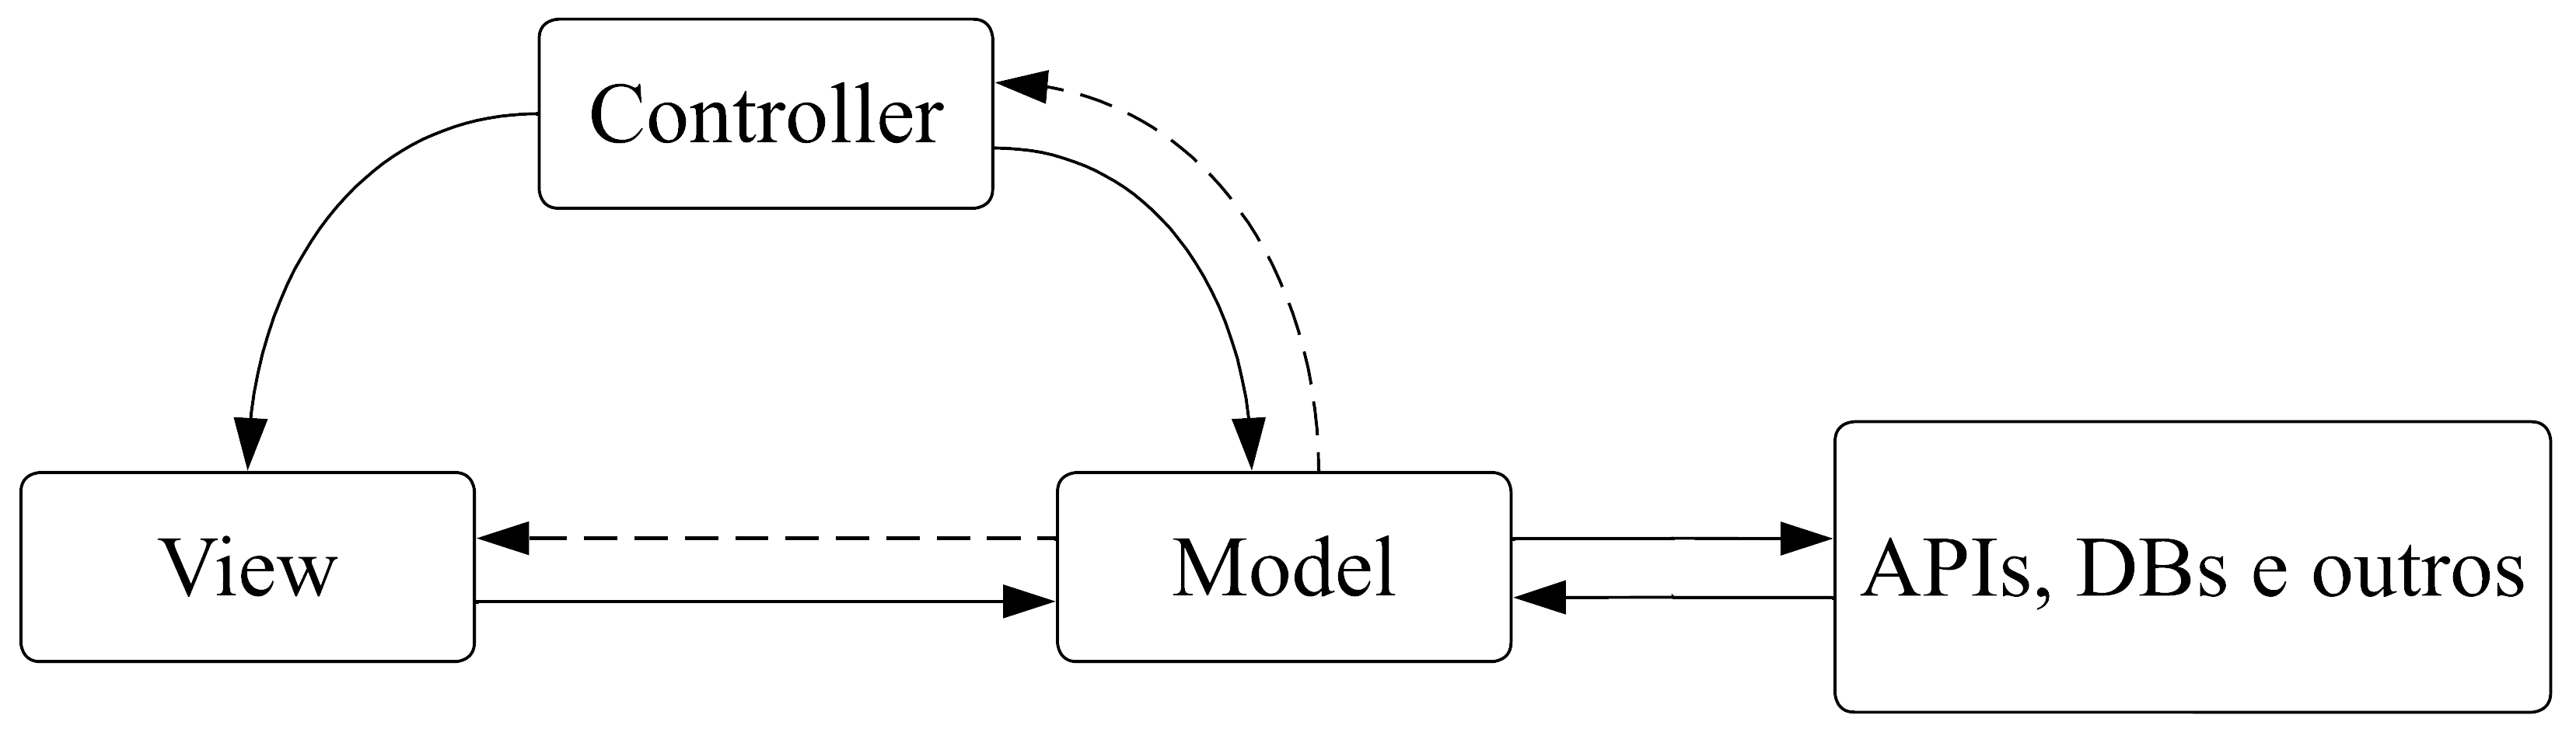
\includegraphics[width=0.52\textwidth]{images/mvc.png}
	\caption{Diagrama do padrão MVC}
	\label{fig:mvc}
\end{figure}

\subsection{A Arquitetura Limpa}

A Arquitetura Limpa é apresentada como uma abordagem que tem por objetivo delimitar responsabilidades para cada um dos componentes em um software.
Esta abordagem produz softwares desacoplados de \emph{frameworks}, interfaces de usuário, bancos de dados e de qualquer agente externo, de modo que as regras de negócio sejam plenamente testáveis~\cite{clean-arch-book}.

A Arquitetura Limpa divide as responsabilidades em quatro níveis: entidades, casos de uso, adaptadores de interfaces e agentes externos.
As entidades encapsulam regras de negócio inerentes ao domínio da aplicação.
Uma entidade pode ser um objeto com métodos, ou um conjunto de estruturas de dados e funções.

Os casos de uso encapsulam as regras específicas para o funcionamento da aplicação.
Eles fazem uso das regras de negócio presentes nas entidades para atingir os seus objetivos.
Não é esperado que mudanças em agentes externos impactem nos casos de uso.

Os adaptadores de interface são componentes responsáveis por converter dados de um formato para outro.
Eles são utilizados, por exemplo, para converter os dados de entidades para um banco de dados ou interface de usuário, e vice-versa.

A camada de agentes externos é composta por \emph{frameworks}, bibliotecas de terceiros, bancos de dados e qualquer outro componente externo que auxilie na execução das regras de negócio.

A Figura~\ref{fig:clean_arch} ilustra as interações entre cada uma das camadas da arquitetura limpa.
Os segmentos de reta tracejados representam uma dependência indireta entre os componentes, isto é, por meio de abstrações.
Já os segmentos de reta contínuos representam uma dependência direta entre os componentes.

\begin{figure}[ht]
	\centering
	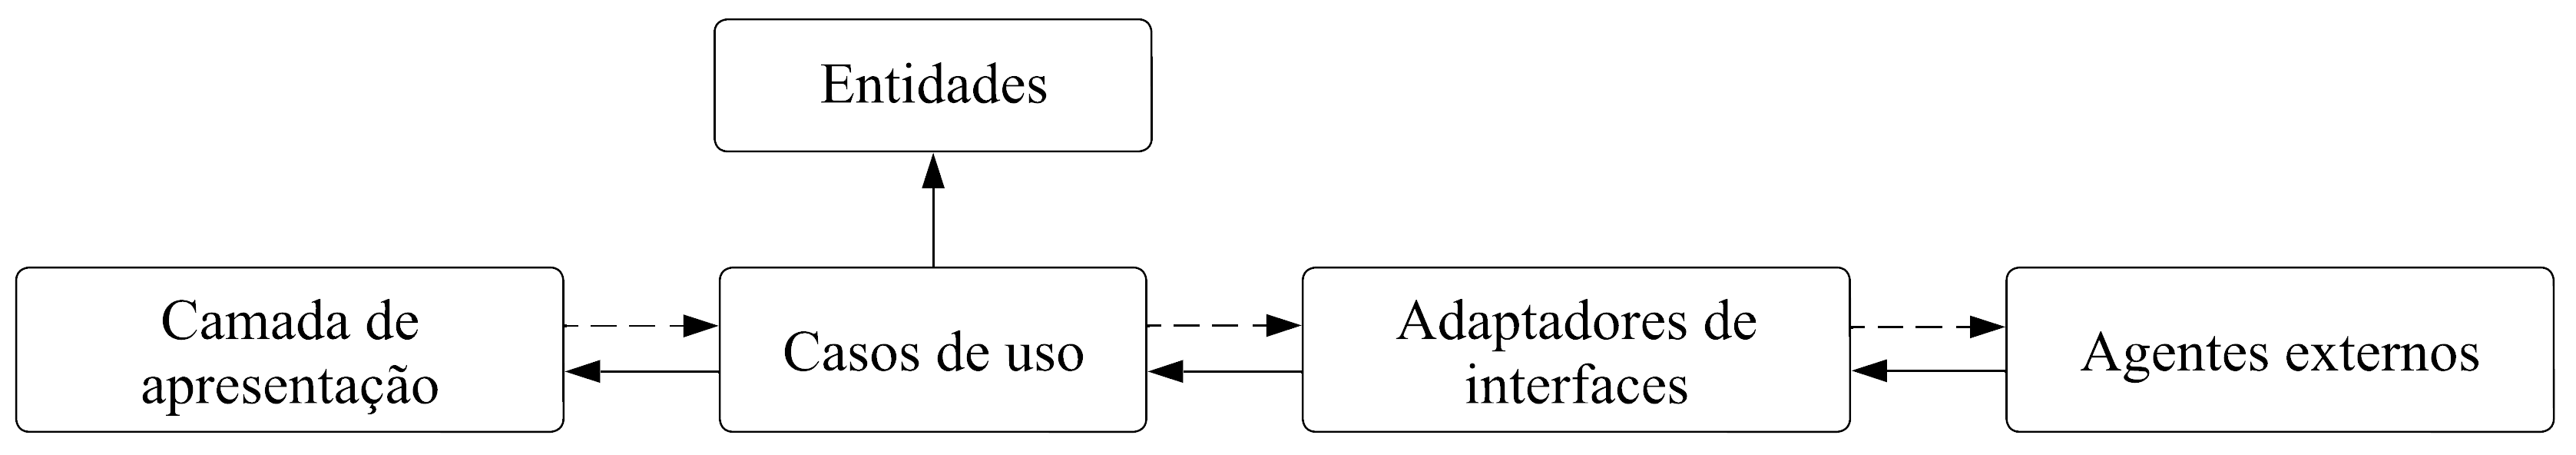
\includegraphics[width=0.9\textwidth]{images/clean_arch.png}
	\caption{Fluxo de funcionamento da Arquitetura Limpa}
	\label{fig:clean_arch}
\end{figure}

Na Figura~\ref{fig:clean_arch_circles} são utilizados círculos concêntricos para representar cada camada.
As camadas mais internas não interagem diretamente com as camadas mais externas.
São utilizadas abstrações para permitir que as camadas se comuniquem, respeitando assim o Princípio de Inversão de Dependências.
Este princípio diz que componentes devem depender de abstrações, e não de implementações concretas.

\begin{figure}[ht]
	\centering
	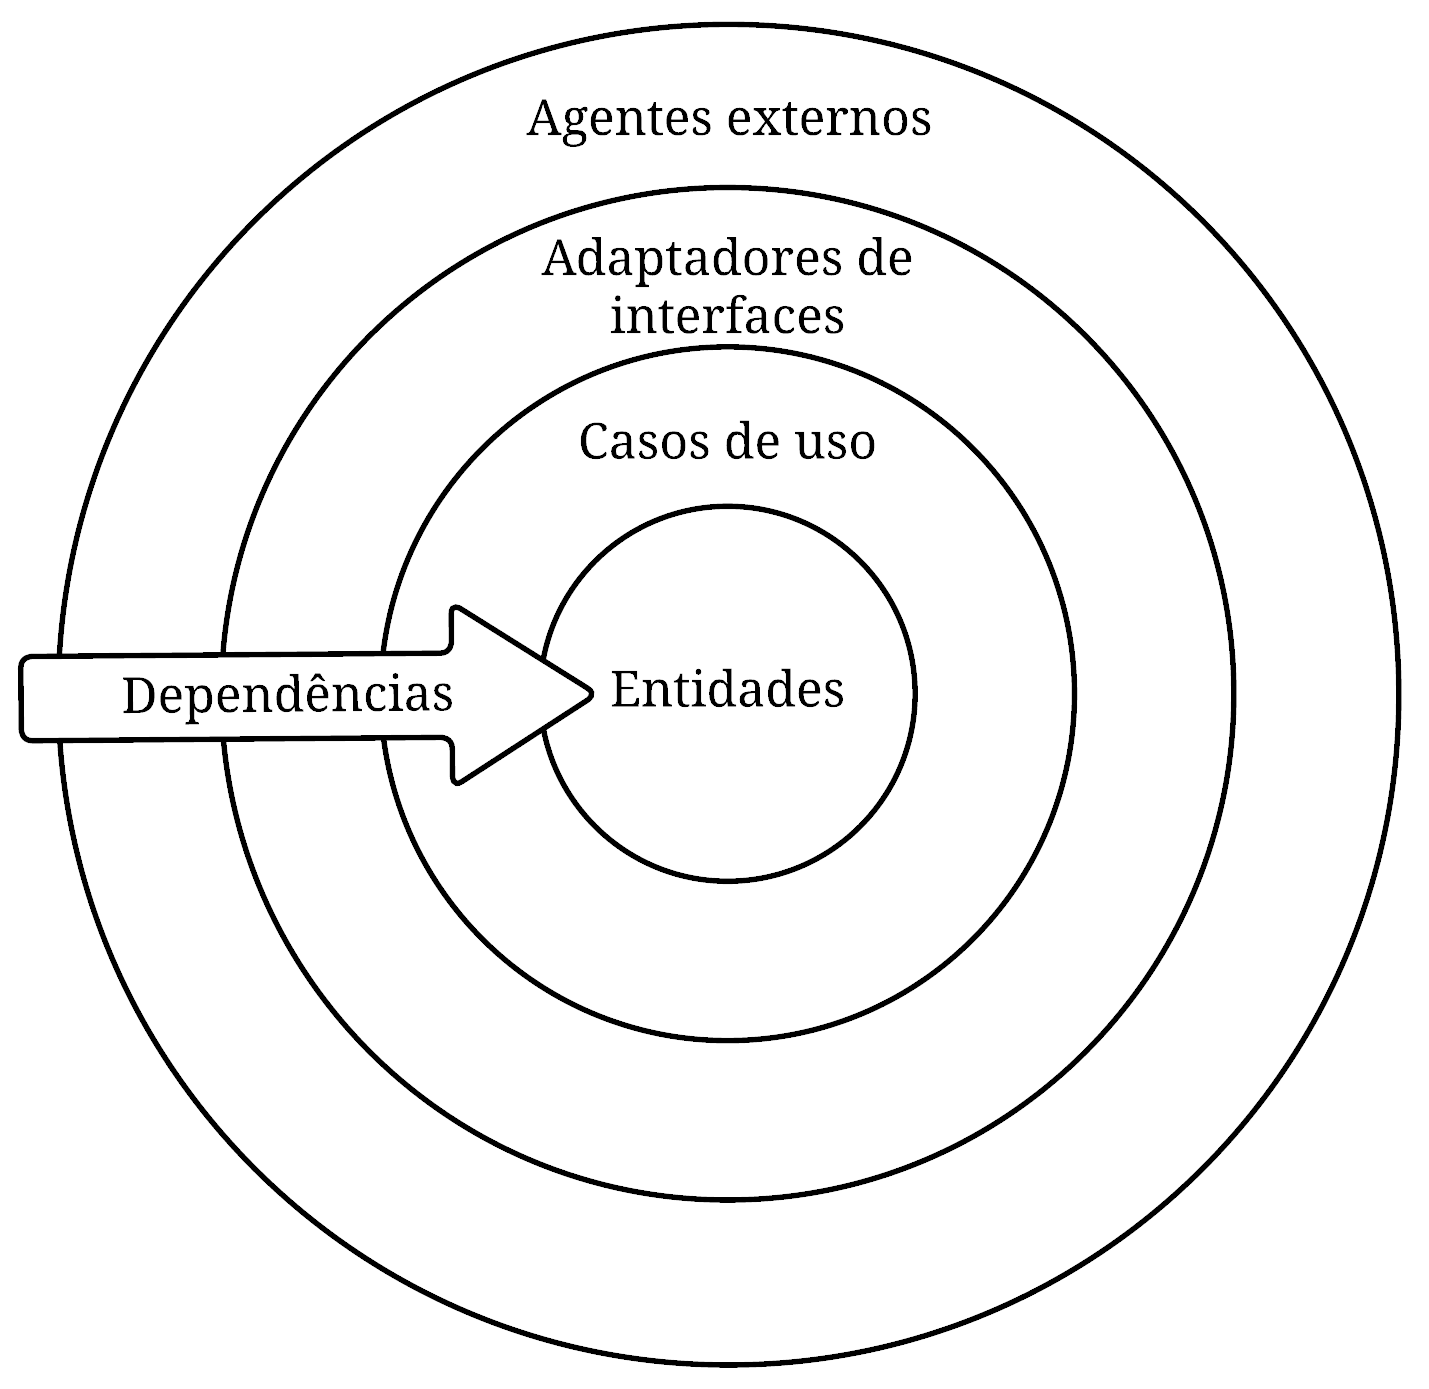
\includegraphics[width=0.65\textwidth]{images/clean_arch_circles.png}
	\caption{Camadas da Arquitetura Limpa e suas dependências}
	\label{fig:clean_arch_circles}
\end{figure}



% Results
\section{Resultados obtidos}

A seguir, são apresentados os resultados obtidos com a análise realizada.

\subsection{Cenário 1: Mudança no banco de dados remoto}

No MVC, as operações relacionadas ao banco de dados remoto se encontram nos \emph{Models}, os quais são \emph{NoteModel} e \emph{UserModel}.
Toda a lógica para obter e adicionar dados está concentrada nestes dois componentes.
Eles fazem uso direto das bibliotecas externas que são necessárias para acessar o Firebase.
Com isso, faz-se necessário alterar esses dois componentes quase que em sua totalidade para se adequarem ao cenário proposto.
Com a alteração destes dois componentes, também seria necessário efetuar modificações nos \emph{Controllers} da aplicação que interagem diretamente com os \emph{Models}.

Na arquitetura limpa, as operações relacionadas ao banco de dados remoto se encontram na camada de agentes externos.
Existem duas classes abstratas que definem operações no banco de dados remotos: \emph{INotesRemoteDataBase} e \emph{IUsersRemoteDataBase}.
Essas duas interfaces possuem suas respectivas implementações utilizando o Firebase.
Os repositórios que fazem uso do banco de dados remoto recebem uma instância das implementações por meio de injeção de dependências, pois estão dependendo de uma abstração, e não de uma implementação concreta.
Para se adequar ao cenário proposto, seria necessário criar implementações de \emph{INotesRemoteDataBase} e \emph{IUsersRemoteDataBase} no novo banco de dados remoto, e realizar a injeção deles na aplicação.
Não é necessário alterar nenhum outro componente além dos que já foram criados anteriormente.

\subsection{Cenário 2: Implementação da pesquisa de notas por título e conteúdo}

No MVC, para adequar-se ao cenário proposto, é necessário criar dois métodos em \emph{NoteModel} para realizar a busca, tanto no banco de dados local como no remoto.
Os dois métodos farão uso direto das bibliotecas externas que são necessárias.
Um terceiro método para ordenar os resultados de forma cronológica também poderá ser criado, e utilizado em ambos os métodos de busca.
Além disso, é necessário criar novos métodos no \emph{Controller} responsável pela listagem de notas, de modo a executar os métodos de busca presentes em \emph{NoteModel}.
A \emph{View} que realiza a listagem de notas também sofrerá alterações.

Já na arquitetura limpa, é necessário criar um novo caso de uso que realize a validação dos dados de entrada do usuário, solicite dados ao repositório das notas e que ao recebê-los, realize a sua ordenação de forma cronológica.
A abstração e implementação do repositório de notas deverão ser modificadas, adicionando-se um método para realização da busca.
O mesmo deve acontecer com as abstrações e implementações dos bancos de dados, que por sua vez, farão uso direto das bibliotecas externas que são necessárias.
Assim como no MVC, é necessário criar novos métodos no \emph{Controller} responsável pela listagem de notas, de modo a consumir o recém criado caso de uso, bem como realizar alterações na \emph{View} correspondente.

\subsection{Cenário 3: Implementação de um novo método de autenticação}

No MVC, as operações relacionadas ao registo e autenticação dos usuários se encontram no \emph{UserModel}.
Ele faz uso das bibliotecas externas que são necessárias para comunicar-se com os serviços de autenticação e o \emph{Firebase}.
Para se adequar ao cenário proposto, é necessário criar um método que realize a autenticação com o \emph{GitHub}.
Também, é necessário adicionar novos métodos no \emph{Controller} que lida com a autenticação para executar o novo método criado.
A \emph{View} que realiza a autenticação também sofrerá modificações.

Na arquitetura limpa, é necessário criar um novo caso de uso que realize a validação dos dados do usuário e encaminhe-os por meio do repositório de autenticação.
Uma abstração e implementação de um serviço que realize a autenticação com o \emph{GitHub} deverão ser criados.
Por sua vez, é necessário modificar a abstração e implementação do repositório de autenticação, incluindo a dependência da abstração do novo serviço criado, bem como um novo método que irá consumir o serviço.
Assim como no MVC, novos métodos serão criados no \emph{Controller} que lida com a autenticação, que passará a consumir o novo caso de uso, além de modificações na \emph{View} correspondente.


% Conclusion
\section{Conclusões}

No presente artigo, o padrão MVC e a arquitetura limpa são comparadas por meio do método de análise de arquiteturas de software baseado em cenários.
São utilizados três cenários: mudanças no banco de dados remoto, implementação da pesquisa de notas por título e conteúdo, e por fim, a implementação de um novo método de autenticação.
Em cada cenário, são observados os componentes que precisam ser criados ou alterados.

Em projetos de pequeno porte, provas de conceito e MVPs (\emph{Minimum Viable Product}, ou produto mínimo viável, em inglês), onde se deseja um rápido desenvolvimento, não se planeja realizar grandes mudanças no futuro, e a regra de negócio não é muito complexa, o MVC se torna uma ótima opção.
Em grandes projetos, onde a aplicação necessita de estabilidade, possui regras de negócio complexas, esteiras de testes unitários, ou até mesmo uma modularização em pequenos pacotes, a arquitetura limpa mostrou-se mais adequada.


% Bibliography
\bibliographystyle{sbc/sbc}
\bibliography{sbc/sbc-template}

\end{document}
